\documentclass[12pt,a4paper]{article}
\usepackage[utf8]{inputenc}
\usepackage{amsmath}
\usepackage{amsfonts}
\usepackage{amssymb}
\usepackage{float}
\usepackage{graphicx}
\author{Darián}
\title{Moogle Informe}
\begin{document}
•INFORME DEL PROYECTO MOOGLE :
\begin{abstract}
Básicamente mi proyecto se basa en la idea de los diccionarios uno como  índice y otro de puntuación de las palabras :
\end{abstract}

\begin{figure}[H]
\centering
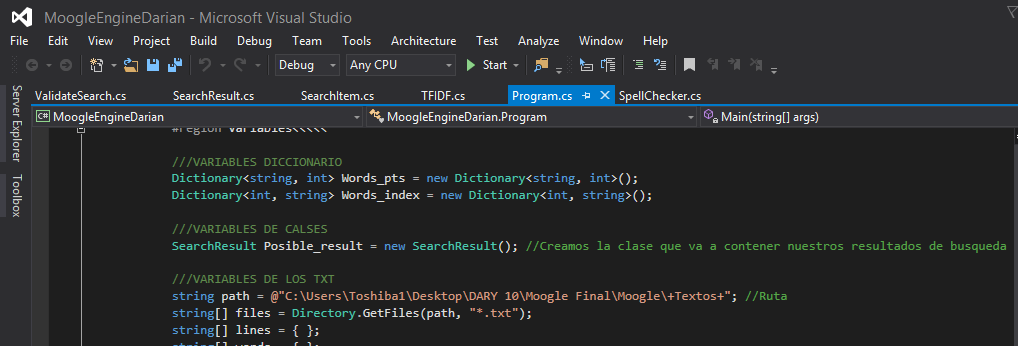
\includegraphics[scale=0.5]{Primero}
\caption{(Esta en el readme pero la ruta se edita en la línea q dice string path)}
\end{figure}
\section{Diccionarios}
$Dictionary<string,int> Words_pts = new Dictionary<string , int >();$
$Dictionary<string,int> Words_index = new Dictionary<string , int >();$
\section{La lógica de los diccionarios funciona a partir }
En el primer foreach( file in files ) , Itera documento por documento y saca todas las líneas del documento actual , dentro de ese foreach:
(Notese que la variable ($dic_index$) es el índice para comenzar a iterar) y eliminamos las líneas vacias del código para evitar iteraciones innecesarias.

En el segundo foreach( line in lines ) , Itera línea por línea, saca los caracteres especiales y pone las palabras divididas de cada línea en un arreglo

En el tercer foreach (words in words), Iteramos las palabras para colocarlas en los diccionarios:
Aquí dentro como vemos creo un if y un else , básicamente lo que digo es que si la palabra existe le sumo 1 , y si no existe la agrego al diccionario .

\section{Clases}
\subsection{$Search_Item$}
El searchitem le hice un pequeño cambio para q devolviera, ademas del snippet , score , title una sugerencia de la palabra(esta parte viene directamente enlazada con el SpellChecker)
\subsection{$Search_Result$}
Recibimos todos los resultados del tipo SearchItem  ,lógicamente con el snippet , score , title y la sugerencia  y el SearchResult  , lo q haria en este caso es colocar en un arreglo todos los posibles resultados , comparo sus scores unos con otros y  reproduzco en pantalla los tres mejores palabras , query(title , snippet , score , suggestion) , basándome en la mejor puntuación.
\subsection{$SpellChecker$}
Inicializo una clase ,busqué hacerlo por una tupla  ósea , q me devolviera dos valores ,  entonces devuelve la palabra a comparar con su puntuación de similitud con la búsqueda .
 Básicamente mi programa se inicializa a través de un if donde si la búsqueda del usuario es diferente a la palabra , comienza la ejecución :
Primero verificamos que la palabra este en el texto, para evitar búsquedas innecesarias, si no está vamos a ir palabra por palabra del diccionario, haciendo comparación
Iterando en el diccionario descarto  las palabras de un solo carácter
Comparo letra por letra:
Si la palabra tiene más de 3 letras en común  la agrego  como un posible resultado de la búsqueda y doy puntos por la similitud de la palabra en el tamaño con la de la búsqueda
Entonces divido la palabra de la búsqueda a la mitad (da un número x) entonces si la palabra con la q la estoy comparando su número de similitudes (es mayor q ese número x) entonces me quedo con la palabra encontrada , en caso contrario con un null

\subsection{$TF-IDF$}
El tf es la frecuencia del término es básicamente la división de la cantidad de veces q aparece la búsqueda sobre la cantidad de palabras en el documento completo.
El idf  es la frecuencia inversa de documento, este valor representa los documentos donde aparezca la palabra sobre la cantidad de documentos totales .
La multiplicación del tf-idf devuelve el score .
Entonces debido al corrector de palabras por cada carácter en común con otra palabra le múltiplico 1000pts al tf de la palabra , en caso de no coincidir la búsqueda con el usuario lo multiplico por -1(para q se vaya al fondo de los scores) , en el caso q la palabra sea exactamente igual a la de la búsqueda le sumo 10000 pts

\subsection{$Validate_Search$}
La idea es revisar q el usuario ponga la búsqueda correctamente y evitar q este ponga menos de 3 caracteres , ya q la búsqueda con dos caracteres , el programa detectaría demasiadas palabras y habrían muchos resultados no deseados.
\section{Snippet}
Anteriormente lo q hacia era reproducir la línea de código donde estaba la palabra y ya está, pero quise mejorarlo entonces mi idea fue iterar sobre la línea donde está la palabra, localizar su índice (en esa línea ósea básicamente si hay una oración "esta casa es... " la palabra esta, mi índice seria,  índice 4 porque es  la posición de su última letra)  entonces ese índice se lo restas al tamaño de la línea, si es menor esa resta q 150 reproduces la línea por pantalla desde la palabra q encontraste, si es mayor q 150 entonces lo reproduces hasta donde llegue la oración en el carácter  150.
\section{El resultado adecuado debe ser: }
\begin{figure}[H]
\centering
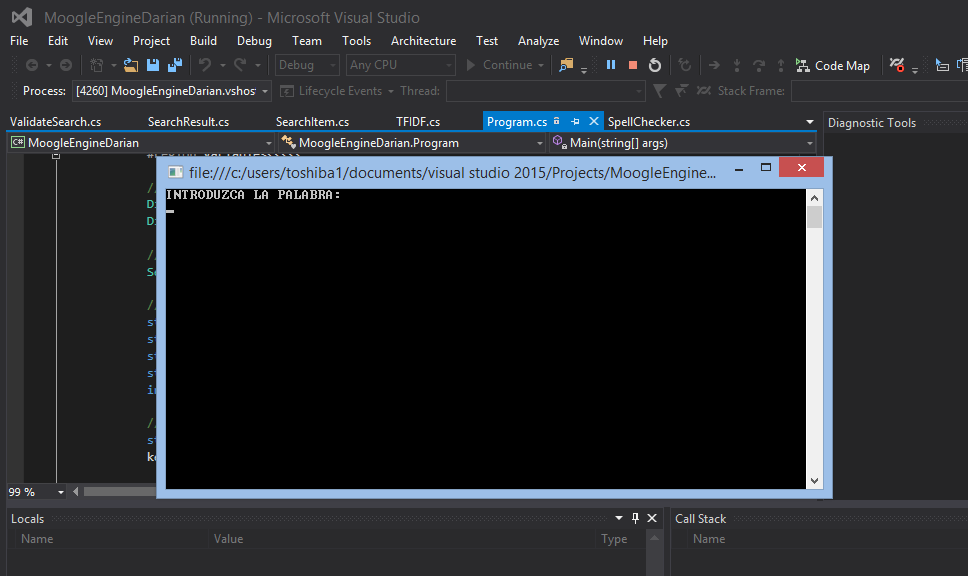
\includegraphics[scale=0.5]{Segundo}
\end{figure}
\section{Casos a probar(ejemplos)}
casa,
años,
literatura
\subsection{Palabras q no tienen los textos , pero reproducen  resultados similares:}
celular ,
pantorilla ,
jamonada

\end{document}